%\documentclass[conference]{IEEEtran}
\documentclass[journal, onecolumn]{IEEEtran}
\IEEEoverridecommandlockouts
% The preceding line is only needed to identify funding in the first footnote. If that is unneeded, please comment it out.
\usepackage{cite}
\usepackage{amsmath,amssymb,amsfonts}
\usepackage{algorithmic}
\usepackage{graphicx}
\usepackage{caption}
\usepackage{textcomp}
\usepackage{diagbox}
\usepackage{subfigure}
\usepackage{epsfig,graphicx,subfigure}
\usepackage{enumitem,balance}
\usepackage{wrapfig}
\usepackage{mathrsfs,euscript}
\usepackage[usenames]{xcolor}
\usepackage{hyperref}
\usepackage{indentfirst}
\usepackage[vlined,ruled,linesnumbered]{algorithm2e}
\def\BibTeX{{\rm B\kern-.05em{\sc i\kern-.025em b}\kern-.08em
    T\kern-.1667em\lower.7ex\hbox{E}\kern-.125emX}}
\begin{document}

\title{Report of Machine Learning Project\\
{\footnotesize Zhixin Ling, 516021910495  \quad  \quad  Yifeng Gao,0000000000000}
\thanks{}
}



\maketitle

\section{Main Ideas}
In this project we use deep methods to perform classification work on Fer2013 dataset. We classify people's face images into seven categories: Angry, Disgust, Fear, Happy, Sad, Surprise and Neutral. We try different network architectures and select network parameters that result in the best accuracy on the given public test set. Finally, we test our networks and parameters on the given private test set to investigate the performance. Also, we try cropping the face segment of the images first to eliminate some unnecessary noises to see whether the classification can improve.

We find networks of ResNet18 and VGG19 achieve the best performance on the given private test dataset with the selected parameters without face cropping. The best resulted accuracy reaches 0.73, reaching the state-of-art achievement. With face cropping, the overall resulted accuracies reduce by about 0.03. However, on several classes, the resulted classification accuracies improve greater than 0.02.

\section{Methods}

\subsection{LeNet}
LeNet is a classical neural network. It is the first complete proposed neural network architecture, including convolution layers, pooling layers, fully connected layers and neuron activation mechanism. A typical version of LeNet is illustrated in \ref{fig:LeNetArch}. The network is simple but can be very effective for some requirements. LeNet's training needs far less computation compared with some later complicate networks. So, LeNet can always worth a try in our classification work.

Compared with the first proposed version of LeNet, we use RELU instead of sigmoid function for neuron activation and also apply batch normalization to ensure a fast and stable convergence.

\subsection{VGG}
VGG, short for Visual Geometry Group Network, is far deeper than LeNet. More convolution kernels are applied; methods of neuron dropout and batch normalization are introduced; larger fully connected layers are used. A typical version of VGG(VGG16) is illustrated in \ref{fig:VGGArch}.
We try several architectures of VGG of different depths to explore whether a deeper network brings a better classification performance.

\subsection{ResNet}
ResNet, short for residual neural network, won the first prize in ILSRVC2015. The special feature of ResNet is that it creatively proposed shortcut connections that allow a former layer to have additional connections, bypassing adjacent layers, leading to the layers behind, as illustrated in \ref{fig:ResNetArch}. The idea greatly ease decreasing of accuracies caused by increasing of network depths, thus allowing the network as deep as possible. As a result, ResNet have far more convolution layers than VGG and also bigger convolution kernels.

\begin{figure}
  \centering
  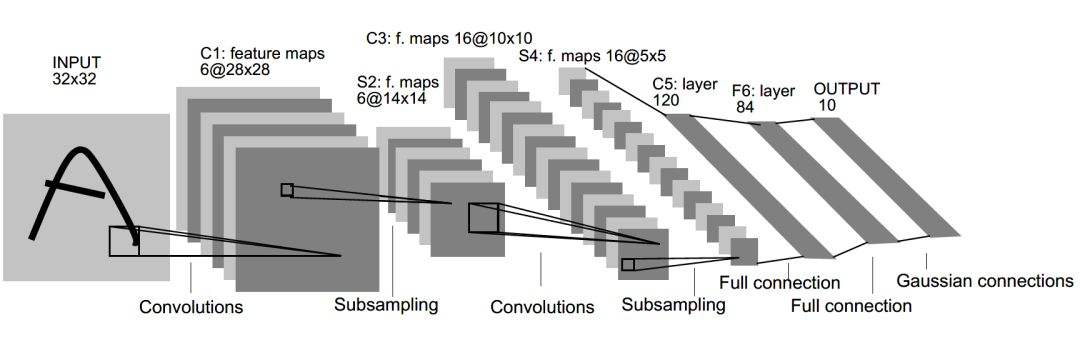
\includegraphics[width=.45\textwidth]{LeNet_the.jpg}
  \caption{Typical Lenet Architecture}
  \label{fig:LeNetArch}
\end{figure}

\begin{figure}
  \centering
  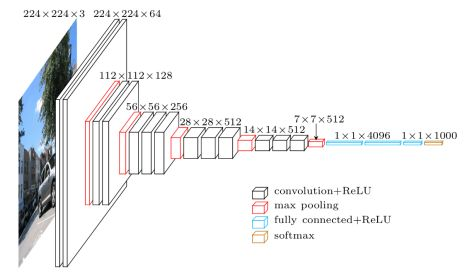
\includegraphics[width=.45\textwidth]{VGG_the.jpg}
  \caption{VGG16 Architecture}
  \label{fig:VGGArch}
\end{figure}

\begin{figure}
  \centering
  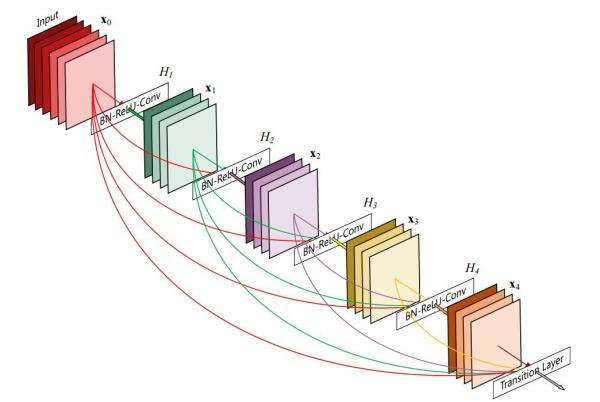
\includegraphics[width=.45\textwidth]{ResNet_the.jpg}
  \caption{Residual Connections}
  \label{fig:ResNetArch}
\end{figure}

\subsection{Face Detection And Cropping}
The samples of our dataset are not all well collected. Faces in some images may be misplaced in a corner and the main contents of the image can be something uncorrelated to the classification work. So we try to detect the area in a image where the face exists and crop the area as a sample. The old image is discarded, of course.
For the work of face detection, we use traditional methods. We use a trained classifier cascaded from strong subclassifiers trained with extracted Haar features of images using Adaboost algorithms.

\subsection{Data Augmentation}
Data augmentation is used to enlarge the training dataset, creating more training samples, to make the trained model more robust and ease overfitting. Symmetry and random cropping are used for data augmentation.


\section{Algorithms}

\subsection{Preprocessing}
Before training, we need to preprocess our data. This includes face detection and cropping, if required, and data augmentation. The algorithm is elaborated in \ref{alg:preprocessing}.

\begin{algorithm}
    \KwIn{ \\
    \quad An $b \times  m$ matrix $B$, a batch of raw data of size $b$. \\
    \quad $F_{DC}$, boolean, whether or not to detect and crop the face part of the image.\\
    \quad $l'$, side length of output image.}
    \KwOut{\\
    \quad A $b \times l' \times l'$ matrix $X$}
    \BlankLine
    \caption{Preprocess}
    \label{alg:preprocessing}
        \For{Every row $R$ in $B$}{
            \tcc{Reshape $R$ to be an image.}
            Reshape $R$ to be an $l \times l$ matrix, where $l = \sqrt{m}$\;
            \If{$F_{DC}$ is true}{
                Detect the area where the face exists in $R$\;
                Discard the rest area of $R$\;
                Resize $R$ to be $l \times l$\;
            }
            \tcc{Perform data augmentation.}
            Randomly select a $l' \times l'$ area in $R$\;
            $R \leftarrow$ the selected part\;
            Randomly decide whether or not to flip the image horizontally with a chance of 0.5\;
        }
        $X \leftarrow B$\;
        \Return{X}\;
\end{algorithm}

\subsection{Network Training}
Because of hardware limitations, we train our model in batches. And learning rate annealing is also applied to stabilize the convergence. After each epoch, we estimate the classification accuracy on the public test set and decide whether or not to save the current network parameters. The algorithm is elaborated in \ref{alg:NetworkTraining}.
\begin{algorithm}
    \KwIn{ \\
    \quad $(X^{tr}, Y^{tr})$, the training set. \\
    \quad $(X^{te}_{pub}, Y^{te}_{pub})$, the public test set. \\
    \quad $F_{DC}$, boolean, whether or not to detect and crop the face part of the image.\\
    \quad $\theta$, parameters of the given network. \\
    \quad $Ep_{m}$, the maximum epoch. \\
    \quad $l'$, side length of image for training. \\
    }
    \KwOut{\\
    \quad $\theta*$, trained parameters of the given network. }
    \BlankLine
    \caption{Network Training}
    \label{alg:NetworkTraining}
        Initialize the $\theta$ and $\theta^* \leftarrow \theta$\;
        Initialize learning rate $l_r$\;
        $acc^{te*}_{pub} \leftarrow 0.0$\;
        \For{$e = 1 \rightarrow Ep_{m}$}{
            \For{Each batch $i$ in $(X^{tr}, Y^{tr})$}{
                Select a batch $(X^{tr}_i, Y^{tr}_i)$ from $(X^{tr}, Y^{tr})$\;
                $Preprocess(X^{tr}_i, F_{DC}, l')$\;
                Calculate array $q$ with $q_j \leftarrow f(\theta, X^{tr}_{i,j})$, where $j = 1,2,\cdots,b$ and $f$ denotes the function corresponding to the given network\;
                $q \leftarrow softmax(q)$\;
                $loss \leftarrow - \frac{1}{b}\sum_{j=1}^{b} Y^{tr}_{i,j} \log q_j$\;
                $\theta \leftarrow - l_r \times \frac{\partial loss}{\partial \theta}$\;
            }
            Calculate $q$ for all batches of $(X^{te}_{pub}, Y^{te}_{pub})$\;
            $acc^{te}_{pub} \leftarrow \frac{1}{s^{te}_{pub}} \sum_{j} argmax(q_j) == Y^{te}_{pub,j} $, where $s^{te}_{pub}$ is total size of public training set\;
            \If{$acc^{te}_{pub} > acc^{te*}_{pub}$}{
                $acc^{te*}_{pub} \leftarrow acc^{te}_{pub}$\;
                $\theta^* \leftarrow \theta$\;
            }
            Anneal $l_r$\;
        }
        \Return{$\theta^*$}\;
\end{algorithm}


\section{Experimental Settings}

\subsection{Convention of Notations}
Before going on, we present our common notations to avoid confusion in table \ref{tab:notations}. The middle column Fixed Value indicates we have a fixed value for the parameter and we use $-$ to indicate the value is not fixed.
 \begin{table}[h]
	\centering
	\caption{Convention of Notations}
	\label{tab:notations}
	\begin{tabular}{ccc}
		\hline
		Notation & Fixed Value & Description \\
		\hline
		\hline
        $l$ & 48 & Side length of raw input images. \\
        $l'$ & 44 & Cropped side length of input images. \\
		$F_{DC}$ & - & Whether or not to detect and crop the face part of the image. \\
        $D_o$ & 0.5 & Neurons' drop out rate when training(if a neuron is allowed so). \\
        $Ep_{m}$ & 250 & Maximum number of epochs. \\
        $l_r(e)$ & $0.01 \times 0.9^{e/5}$ & Learning rate in a given epoch $e$. \\
        $b$ & - & Batch size. \\
        $S_{tr}=(X^{tr}, Y^{tr})$ & \checkmark & Training set. \\
        $S_{pub}=(X^{te}_{pub}, Y^{te}_{pub})$ & \checkmark & Public test set. \\
        $S_{pri}=(X^{te}_{pri}, Y^{te}_{pri})$ & \checkmark & Private test set. \\
        $acc^{tr}(e)$ & - & Training accuracy in a given epoch $e$. \\
        $acc^{te}_{pub}(e)$ & - & Private test accuracy in a given epoch $e$. \\
        $acc^{te}_{pri}(e)$ & - & Public test accuracy in a given epoch $e$. \\
		\hline
	\end{tabular}
\end{table}

\subsection{Detailed Network Structures}
We conduct eight experiments with different settings on six different networks. We use LetNet5, VGG11, VGG13, VGG16, VGG19 and ResNet18, as shown in table \ref{tab:LeNet5-VGG} and figure \ref{fig:ResNet18}.  In table \ref{tab:LeNet5-VGG}, we denote a convolution layer as "conv<kernel size>-<kernel numbers>" and a fully connected layer as "FC-<neuron numbers>". RELU is used for neuron activation. Padding is applied with every convolution layers and batch normalization is used after convolution.

Compared with the LeNet5 structure used for mnist digits classification, we adjust the fully connected layers to adapt to our dataset and apply batch normalization.

Compared with standard VGG structures proposed by Karen Simonyan, et al., we, use only one fully connected layer("FC-512") after convolution layers except the output layer while Karen Simonyan, et al. use two 4096-neuron layers. We do not need such complicated fully connected layers because we have only seven classes while they have one thousand.

Since ResNet is more difficult to describe, we turn to tensorboard for visualization. The detailed parameters are elaborated in \ref{tab:ResNet18}. We denote a convolution layer using $n$ $s$-sized kernels as ($s$, $n$) and $a$ sequenced building blocks composed of $k$ convolution layer as [($s_1$, $n_1$),($s_2$, $n_2$), $\cdots$, ($s_k$, $n_k$)] $\times a$. Within every building block, there is a residual connection from block input to block output, bypassing the contained convolution layers, as illustrated in the right block of figure \ref{fig:ResNet18}.

For every fully connected layer, we drop out the neurons with a rate of $D_o=0.5$.

\begin{table}
%\Large
\caption{Structures of LeNet5 and VGG}
\label{tab:LeNet5-VGG}
\begin{center}
\begin{tabular}{|c|c|c|c|c| p{5cm}|}
\hline
LeNet5 & VGG11      & VGG13         & VGG16     & VGG19  \\ \hline 
input & input & input               & input & input  \\  
conv5-6 & conv3-64   & conv3-64     & conv3-64  & conv3-64  \\
maxpool & maxpool & conv3-64        & conv3-64 & conv3-64  \\  
conv5-16 & conv3-128 & maxpool      & maxpool  & maxpool  \\  
maxpool & maxpool & conv3-128       & conv3-128 & conv3-128  \\  
FC-144 & conv3-256 & conv3-128      & conv3-128 & conv3-128  \\  
FC-84 & conv3-256 & maxpool         & maxpool & maxpool  \\  
FC-7 & maxpool & conv3-256          & conv3-256 & conv3-256  \\  
soft-max & conv3-512 & conv3-256    & conv3-256 & conv3-256  \\
 & conv3-512 & maxpool              & conv3-256 & conv3-256  \\  
 & maxpool & conv3-512              & maxpool & conv3-256  \\  
 & conv3-512 & conv3-512            & conv3-512 & maxpool  \\
 & conv3-512 & maxpool              & conv3-512 & conv3-512  \\  
 & maxpool & conv3-512              & conv3-512 & conv3-512  \\
 & FC-512  & conv3-512              & maxpool & conv3-512  \\  
 &FC-7 & maxpool                 & conv3-512 & conv3-512  \\  
 & soft-max &    FC-512                & conv3-512 & maxpool  \\  
 &  &  FC-7                & conv3-512 & conv3-512  \\   
  &  &  soft-max                        & maxpool & conv3-512  \\
   &  &                    & FC-512 & conv3-512  \\
    &  &                            & FC-7 & conv3-512  \\  
  &  &                          &      soft-max     & maxpool  \\
   &  &                     &               & FC-512   \\
    &  &                            &       & FC-7  \\  
        &  &                        &       & soft-max \\  \hline 
\end{tabular}
\end{center}
\end{table}  

\begin{table}
%\Large
\caption{Structures of ResNet18}
\label{tab:ResNet18}
\begin{center}
\begin{tabular}{|c|c| p{5cm}|}
\hline
Layer Name & Blocks    \\ \hline
conv1 & (3,64)   \\
conv2.x    & $[(3,128),(3,128)] \times 2$  \\  
conv3.x    & $[(3,256),(3,256)] \times 2$  \\  
conv4.x    & $[(3,512),(3,512)] \times 2$  \\  
FC1    & FC-512  \\  
output    & soft-max  \\   \hline
\end{tabular}
\end{center}
\end{table}  

\begin{figure}
  \centering
  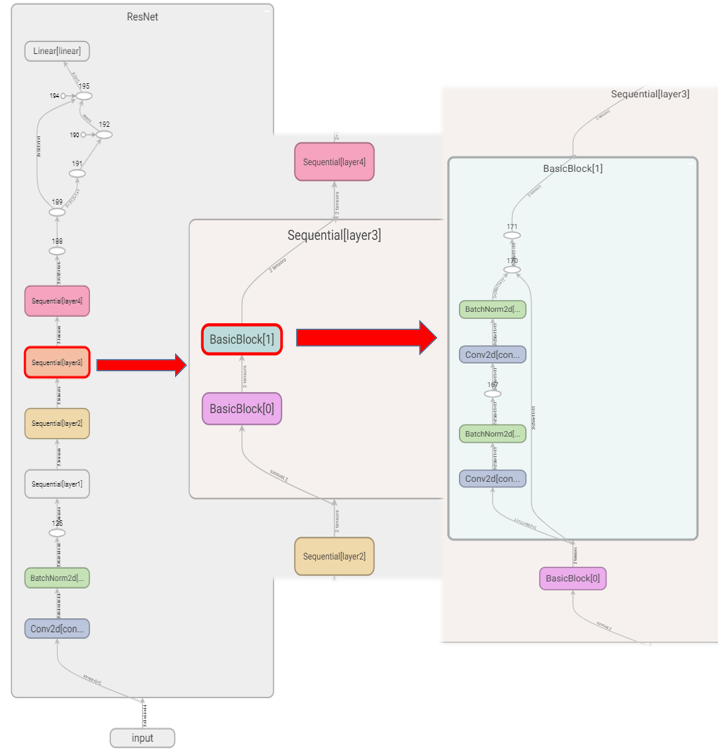
\includegraphics[width=.5\textwidth]{ResNet18_2.png}
  \caption{Structures of ResNet18}
  \label{fig:ResNet18}
\end{figure}


\subsection{Hyper-Parameters of Experiments}
We conduct seven experiments regard of different networks, whether or not crop faces in preprocessing and the batch size used for training. The details are illustrated in table \ref{tab:Hps}.
\begin{table}
%\Large
\caption{Hyper-Parameters of Experiments}
\label{tab:Hps}
\begin{center}
\begin{tabular}{|c|c|c|c|c|c|c|c| p{1.5cm}|}
\hline
Experiment Name & ExLenet5 & ExLenet5-DC & ExVGG11 & ExVGG13 & ExVGG16 & ExVGG19 & ExVGG19-DC & ExRes18    \\ \hline
$F_{DC}$  & $\times$ & \checkmark & $\times$ & $\times$ & $\times$ & $\times$ & \checkmark & $\times$  \\ \hline
$b$    & 64 & 64 & 64 & 64 & 64 & 64 & 64 & 32  \\ \hline
Network    & Lenet5 & Lenet5 & VGG11 & VGG13 & VGG16 & VGG19 & VGG19 & ResNet18  \\  \hline
\end{tabular}
\end{center}
\end{table} 



\section{Results}
Results.


\end{document}





